% Graphic for TeX using PGF
% Title: /home/james/src/ML@B/alexa/architechture.dia
% Creator: Dia v0.97.3
% CreationDate: Fri Oct 28 17:15:29 2016
% For: james
% \usepackage{tikz}
% The following commands are not supported in PSTricks at present
% We define them conditionally, so when they are implemented,
% this pgf file will use them.
\ifx\du\undefined
  \newlength{\du}
\fi
\setlength{\du}{15\unitlength}
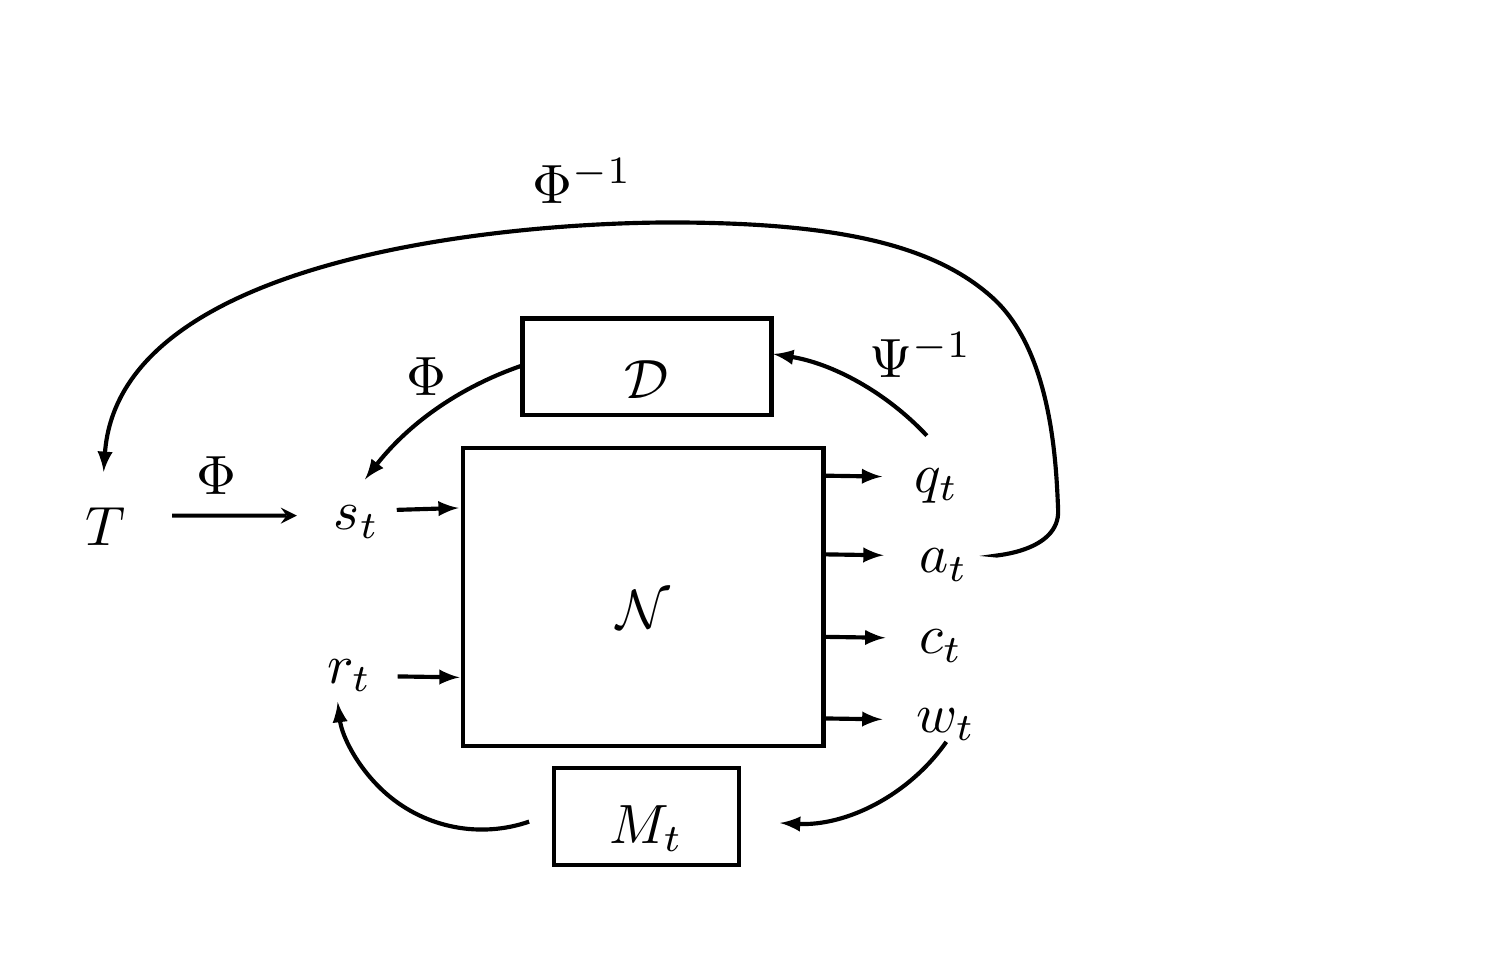
\begin{tikzpicture}
\pgftransformxscale{1.000000}
\pgftransformyscale{-1.000000}
\definecolor{dialinecolor}{rgb}{0.000000, 0.000000, 0.000000}
\pgfsetstrokecolor{dialinecolor}
\definecolor{dialinecolor}{rgb}{1.000000, 1.000000, 1.000000}
\pgfsetfillcolor{dialinecolor}
% setfont left to latex
\definecolor{dialinecolor}{rgb}{0.000000, 0.000000, 0.000000}
\pgfsetstrokecolor{dialinecolor}
\node[anchor=west] at (25.077276\du,36.891499\du){\scalebox{2}{$\mathfrak{T}$}};
\pgfsetlinewidth{0.100000\du}
\pgfsetdash{}{0pt}
\pgfsetdash{}{0pt}
\pgfsetbuttcap
{
\definecolor{dialinecolor}{rgb}{0.000000, 0.000000, 0.000000}
\pgfsetfillcolor{dialinecolor}
% was here!!!
\pgfsetarrowsend{stealth}
\definecolor{dialinecolor}{rgb}{0.000000, 0.000000, 0.000000}
\pgfsetstrokecolor{dialinecolor}
\draw (27.401006\du,36.627037\du)--(30.404188\du,36.627238\du);
}
% setfont left to latex
\definecolor{dialinecolor}{rgb}{0.000000, 0.000000, 0.000000}
\pgfsetstrokecolor{dialinecolor}
\node[anchor=west] at (27.721957\du,35.664185\du){\scalebox{2}{$\Phi$}};
\definecolor{dialinecolor}{rgb}{1.000000, 1.000000, 1.000000}
\pgfsetfillcolor{dialinecolor}
\fill (34.407656\du,35.007860\du)--(34.407656\du,42.175101\du)--(43.090156\du,42.175101\du)--(43.090156\du,35.007860\du)--cycle;
\pgfsetlinewidth{0.100000\du}
\pgfsetdash{}{0pt}
\pgfsetdash{}{0pt}
\pgfsetmiterjoin
\definecolor{dialinecolor}{rgb}{0.000000, 0.000000, 0.000000}
\pgfsetstrokecolor{dialinecolor}
\draw (34.407656\du,35.007860\du)--(34.407656\du,42.175101\du)--(43.090156\du,42.175101\du)--(43.090156\du,35.007860\du)--cycle;
% setfont left to latex
\definecolor{dialinecolor}{rgb}{0.000000, 0.000000, 0.000000}
\pgfsetstrokecolor{dialinecolor}
\node at (38.748906\du,38.891619\du){\scalebox{2}{$\mathcal{N}$}};
% setfont left to latex
\definecolor{dialinecolor}{rgb}{0.000000, 0.000000, 0.000000}
\pgfsetstrokecolor{dialinecolor}
\node[anchor=west] at (38.748906\du,38.591480\du){};
% setfont left to latex
\definecolor{dialinecolor}{rgb}{0.000000, 0.000000, 0.000000}
\pgfsetstrokecolor{dialinecolor}
\node[anchor=west] at (38.693568\du,42.573271\du){};
% setfont left to latex
\definecolor{dialinecolor}{rgb}{0.000000, 0.000000, 0.000000}
\pgfsetstrokecolor{dialinecolor}
\node[anchor=west] at (41.247737\du,30.552100\du){};
% setfont left to latex
\definecolor{dialinecolor}{rgb}{0.000000, 0.000000, 0.000000}
\pgfsetstrokecolor{dialinecolor}
\node[anchor=west] at (35.814500\du,28.557621\du){\scalebox{2}{$\Phi^{-1}$}};
% setfont left to latex
\definecolor{dialinecolor}{rgb}{0.000000, 0.000000, 0.000000}
\pgfsetstrokecolor{dialinecolor}
\node[anchor=west] at (31.046089\du,32.569504\du){};
% setfont left to latex
\definecolor{dialinecolor}{rgb}{0.000000, 0.000000, 0.000000}
\pgfsetstrokecolor{dialinecolor}
\node[anchor=west] at (30.885614\du,31.904678\du){};
% setfont left to latex
\definecolor{dialinecolor}{rgb}{0.000000, 0.000000, 0.000000}
\pgfsetstrokecolor{dialinecolor}
\node[anchor=west] at (38.748906\du,38.591480\du){};
% setfont left to latex
\definecolor{dialinecolor}{rgb}{0.000000, 0.000000, 0.000000}
\pgfsetstrokecolor{dialinecolor}
\node[anchor=west] at (41.396749\du,46.649736\du){};
% setfont left to latex
\definecolor{dialinecolor}{rgb}{0.000000, 0.000000, 0.000000}
\pgfsetstrokecolor{dialinecolor}
\node[anchor=west] at (45.007445\du,35.916562\du){\scalebox{2}{$q_t$}};
% setfont left to latex
\definecolor{dialinecolor}{rgb}{0.000000, 0.000000, 0.000000}
\pgfsetstrokecolor{dialinecolor}
\node[anchor=west] at (45.122070\du,37.819341\du){\scalebox{2}{$a_t$}};
% setfont left to latex
\definecolor{dialinecolor}{rgb}{0.000000, 0.000000, 0.000000}
\pgfsetstrokecolor{dialinecolor}
\node[anchor=west] at (45.124363\du,39.773797\du){\scalebox{2}{$c_t$}};
% setfont left to latex
\definecolor{dialinecolor}{rgb}{0.000000, 0.000000, 0.000000}
\pgfsetstrokecolor{dialinecolor}
\node[anchor=west] at (45.053295\du,41.670749\du){\scalebox{2}{$w_t$}};
\pgfsetlinewidth{0.100000\du}
\pgfsetdash{}{0pt}
\pgfsetdash{}{0pt}
\pgfsetbuttcap
{
\definecolor{dialinecolor}{rgb}{0.000000, 0.000000, 0.000000}
\pgfsetfillcolor{dialinecolor}
% was here!!!
\pgfsetarrowsend{latex}
\definecolor{dialinecolor}{rgb}{0.000000, 0.000000, 0.000000}
\pgfsetstrokecolor{dialinecolor}
\draw (43.035891\du,35.664386\du)--(44.503094\du,35.687311\du);
}
\pgfsetlinewidth{0.100000\du}
\pgfsetdash{}{0pt}
\pgfsetdash{}{0pt}
\pgfsetbuttcap
{
\definecolor{dialinecolor}{rgb}{0.000000, 0.000000, 0.000000}
\pgfsetfillcolor{dialinecolor}
% was here!!!
\pgfsetarrowsend{latex}
\definecolor{dialinecolor}{rgb}{0.000000, 0.000000, 0.000000}
\pgfsetstrokecolor{dialinecolor}
\draw (43.043108\du,41.512730\du)--(44.510311\du,41.535655\du);
}
\pgfsetlinewidth{0.100000\du}
\pgfsetdash{}{0pt}
\pgfsetdash{}{0pt}
\pgfsetbuttcap
{
\definecolor{dialinecolor}{rgb}{0.000000, 0.000000, 0.000000}
\pgfsetfillcolor{dialinecolor}
% was here!!!
\pgfsetarrowsend{latex}
\definecolor{dialinecolor}{rgb}{0.000000, 0.000000, 0.000000}
\pgfsetstrokecolor{dialinecolor}
\draw (43.114176\du,39.548053\du)--(44.581379\du,39.570978\du);
}
\pgfsetlinewidth{0.100000\du}
\pgfsetdash{}{0pt}
\pgfsetdash{}{0pt}
\pgfsetbuttcap
{
\definecolor{dialinecolor}{rgb}{0.000000, 0.000000, 0.000000}
\pgfsetfillcolor{dialinecolor}
% was here!!!
\pgfsetarrowsend{latex}
\definecolor{dialinecolor}{rgb}{0.000000, 0.000000, 0.000000}
\pgfsetstrokecolor{dialinecolor}
\draw (43.070618\du,37.560451\du)--(44.537821\du,37.583376\du);
}
% setfont left to latex
\definecolor{dialinecolor}{rgb}{0.000000, 0.000000, 0.000000}
\pgfsetstrokecolor{dialinecolor}
\node[anchor=west] at (31.023164\du,36.787714\du){\scalebox{2}{$s_t$}};
\pgfsetlinewidth{0.100000\du}
\pgfsetdash{}{0pt}
\pgfsetdash{}{0pt}
\pgfsetbuttcap
{
\definecolor{dialinecolor}{rgb}{0.000000, 0.000000, 0.000000}
\pgfsetfillcolor{dialinecolor}
% was here!!!
\pgfsetarrowsend{latex}
\definecolor{dialinecolor}{rgb}{0.000000, 0.000000, 0.000000}
\pgfsetstrokecolor{dialinecolor}
\draw (32.811318\du,36.489688\du)--(34.301446\du,36.443838\du);
}
\pgfsetlinewidth{0.100000\du}
\pgfsetdash{}{0pt}
\pgfsetdash{}{0pt}
\pgfsetbuttcap
{
\definecolor{dialinecolor}{rgb}{0.000000, 0.000000, 0.000000}
\pgfsetfillcolor{dialinecolor}
% was here!!!
\pgfsetarrowsend{latex}
\definecolor{dialinecolor}{rgb}{0.000000, 0.000000, 0.000000}
\pgfsetstrokecolor{dialinecolor}
\draw (32.834243\du,40.501572\du)--(34.324371\du,40.524497\du);
}
% setfont left to latex
\definecolor{dialinecolor}{rgb}{0.000000, 0.000000, 0.000000}
\pgfsetstrokecolor{dialinecolor}
\node[anchor=west] at (30.862689\du,40.478647\du){\scalebox{2}{$r_t$}};
% setfont left to latex
\definecolor{dialinecolor}{rgb}{0.000000, 0.000000, 0.000000}
\pgfsetstrokecolor{dialinecolor}
\node[anchor=west] at (23.870548\du,36.099962\du){};
% setfont left to latex
\definecolor{dialinecolor}{rgb}{0.000000, 0.000000, 0.000000}
\pgfsetstrokecolor{dialinecolor}
\node[anchor=west] at (28.478483\du,35.572686\du){};
\pgfsetlinewidth{0.100000\du}
\pgfsetdash{}{0pt}
\pgfsetdash{}{0pt}
\pgfsetbuttcap
{
\definecolor{dialinecolor}{rgb}{0.000000, 0.000000, 0.000000}
\pgfsetfillcolor{dialinecolor}
% was here!!!
\pgfsetarrowsend{latex}
\definecolor{dialinecolor}{rgb}{0.000000, 0.000000, 0.000000}
\pgfsetstrokecolor{dialinecolor}
\pgfpathmoveto{\pgfpoint{45.580628\du}{34.701594\du}}
\pgfpatharc{317}{279}{6.434495\du and 6.434495\du}
\pgfusepath{stroke}
}
\pgfsetlinewidth{0.100000\du}
\pgfsetdash{}{0pt}
\pgfsetdash{}{0pt}
\pgfsetbuttcap
{
\definecolor{dialinecolor}{rgb}{0.000000, 0.000000, 0.000000}
\pgfsetfillcolor{dialinecolor}
% was here!!!
\pgfsetarrowsend{latex}
\definecolor{dialinecolor}{rgb}{0.000000, 0.000000, 0.000000}
\pgfsetstrokecolor{dialinecolor}
\pgfpathmoveto{\pgfpoint{38.634503\du}{32.542226\du}}
\pgfpatharc{270}{218}{8.360154\du and 8.360154\du}
\pgfusepath{stroke}
}
% setfont left to latex
\definecolor{dialinecolor}{rgb}{0.000000, 0.000000, 0.000000}
\pgfsetstrokecolor{dialinecolor}
\node[anchor=west] at (43.929967\du,32.752905\du){\scalebox{2}{$\Psi^{-1}$}};
% setfont left to latex
\definecolor{dialinecolor}{rgb}{0.000000, 0.000000, 0.000000}
\pgfsetstrokecolor{dialinecolor}
\node[anchor=west] at (32.765468\du,33.280181\du){\scalebox{2}{$\Phi$}};
% setfont left to latex
\definecolor{dialinecolor}{rgb}{0.000000, 0.000000, 0.000000}
\pgfsetstrokecolor{dialinecolor}
\node[anchor=west] at (27.721957\du,39.424095\du){};
% setfont left to latex
\definecolor{dialinecolor}{rgb}{0.000000, 0.000000, 0.000000}
\pgfsetstrokecolor{dialinecolor}
\node[anchor=west] at (36.960752\du,30.116524\du){};
% setfont left to latex
\definecolor{dialinecolor}{rgb}{0.000000, 0.000000, 0.000000}
\pgfsetstrokecolor{dialinecolor}
\node[anchor=west] at (58.097649\du,25.095938\du){};
\definecolor{dialinecolor}{rgb}{1.000000, 1.000000, 1.000000}
\pgfsetfillcolor{dialinecolor}
\fill (35.841856\du,31.879218\du)--(35.841856\du,34.213940\du)--(41.839356\du,34.213940\du)--(41.839356\du,31.879218\du)--cycle;
\pgfsetlinewidth{0.100000\du}
\pgfsetdash{}{0pt}
\pgfsetdash{}{0pt}
\pgfsetmiterjoin
\definecolor{dialinecolor}{rgb}{0.000000, 0.000000, 0.000000}
\pgfsetstrokecolor{dialinecolor}
\draw (35.841856\du,31.879218\du)--(35.841856\du,34.213940\du)--(41.839356\du,34.213940\du)--(41.839356\du,31.879218\du)--cycle;
% setfont left to latex
\definecolor{dialinecolor}{rgb}{0.000000, 0.000000, 0.000000}
\pgfsetstrokecolor{dialinecolor}
\node at (38.840606\du,33.346718\du){\scalebox{2}{$\mathcal{D}$}};
% setfont left to latex
\definecolor{dialinecolor}{rgb}{0.000000, 0.000000, 0.000000}
\pgfsetstrokecolor{dialinecolor}
\node[anchor=west] at (38.840606\du,33.046579\du){};
% setfont left to latex
\definecolor{dialinecolor}{rgb}{0.000000, 0.000000, 0.000000}
\pgfsetstrokecolor{dialinecolor}
\node[anchor=west] at (35.841856\du,32.462899\du){};
% setfont left to latex
\definecolor{dialinecolor}{rgb}{0.000000, 0.000000, 0.000000}
\pgfsetstrokecolor{dialinecolor}
\node[anchor=west] at (32.788393\du,32.569504\du){};
\definecolor{dialinecolor}{rgb}{1.000000, 1.000000, 1.000000}
\pgfsetfillcolor{dialinecolor}
\fill (36.593951\du,42.699842\du)--(36.593951\du,45.034564\du)--(41.064336\du,45.034564\du)--(41.064336\du,42.699842\du)--cycle;
\pgfsetlinewidth{0.100000\du}
\pgfsetdash{}{0pt}
\pgfsetdash{}{0pt}
\pgfsetmiterjoin
\definecolor{dialinecolor}{rgb}{0.000000, 0.000000, 0.000000}
\pgfsetstrokecolor{dialinecolor}
\draw (36.593951\du,42.699842\du)--(36.593951\du,45.034564\du)--(41.064336\du,45.034564\du)--(41.064336\du,42.699842\du)--cycle;
% setfont left to latex
\definecolor{dialinecolor}{rgb}{0.000000, 0.000000, 0.000000}
\pgfsetstrokecolor{dialinecolor}
\node at (38.829144\du,44.167342\du){\scalebox{2}{$M_t$}};
% setfont left to latex
\definecolor{dialinecolor}{rgb}{0.000000, 0.000000, 0.000000}
\pgfsetstrokecolor{dialinecolor}
\node[anchor=west] at (26.529854\du,36.741864\du){};
% setfont left to latex
\definecolor{dialinecolor}{rgb}{0.000000, 0.000000, 0.000000}
\pgfsetstrokecolor{dialinecolor}
\node[anchor=west] at (25.154351\du,36.925264\du){};
% setfont left to latex
\definecolor{dialinecolor}{rgb}{0.000000, 0.000000, 0.000000}
\pgfsetstrokecolor{dialinecolor}
\node[anchor=west] at (31.642140\du,40.386947\du){};
% setfont left to latex
\definecolor{dialinecolor}{rgb}{0.000000, 0.000000, 0.000000}
\pgfsetstrokecolor{dialinecolor}
\node[anchor=west] at (44.480169\du,33.371881\du){};
% setfont left to latex
\definecolor{dialinecolor}{rgb}{0.000000, 0.000000, 0.000000}
\pgfsetstrokecolor{dialinecolor}
\node[anchor=west] at (31.435815\du,36.650163\du){};
\pgfsetlinewidth{0.100000\du}
\pgfsetdash{}{0pt}
\pgfsetdash{}{0pt}
\pgfsetmiterjoin
\pgfsetbuttcap
{
\definecolor{dialinecolor}{rgb}{0.000000, 0.000000, 0.000000}
\pgfsetfillcolor{dialinecolor}
% was here!!!
\pgfsetarrowsend{latex}
\definecolor{dialinecolor}{rgb}{0.000000, 0.000000, 0.000000}
\pgfsetstrokecolor{dialinecolor}
\pgfpathmoveto{\pgfpoint{47.277025\du}{37.590091\du}}
\pgfpathcurveto{\pgfpoint{47.109580\du}{37.590091\du}}{\pgfpoint{48.790078\du}{37.521315\du}}{\pgfpoint{48.744228\du}{36.489688\du}}
\pgfpathcurveto{\pgfpoint{48.698378\du}{35.458061\du}}{\pgfpoint{48.614319\du}{32.687951\du}}{\pgfpoint{47.162400\du}{31.377402\du}}
\pgfpathcurveto{\pgfpoint{45.710480\du}{30.066853\du}}{\pgfpoint{43.333916\du}{29.589248\du}}{\pgfpoint{39.620058\du}{29.566323\du}}
\pgfpathcurveto{\pgfpoint{35.906200\du}{29.543398\du}}{\pgfpoint{26.117203\du}{30.276999\du}}{\pgfpoint{25.750402\du}{35.572686\du}}
\pgfusepath{stroke}
}
\pgfsetlinewidth{0.100000\du}
\pgfsetdash{}{0pt}
\pgfsetdash{}{0pt}
\pgfsetbuttcap
{
\definecolor{dialinecolor}{rgb}{0.000000, 0.000000, 0.000000}
\pgfsetfillcolor{dialinecolor}
% was here!!!
\pgfsetarrowsend{latex}
\definecolor{dialinecolor}{rgb}{0.000000, 0.000000, 0.000000}
\pgfsetstrokecolor{dialinecolor}
\pgfpathmoveto{\pgfpoint{46.049754\du}{42.077865\du}}
\pgfpatharc{35}{93}{4.596556\du and 4.596556\du}
\pgfusepath{stroke}
}
\pgfsetlinewidth{0.100000\du}
\pgfsetdash{}{0pt}
\pgfsetdash{}{0pt}
\pgfsetbuttcap
{
\definecolor{dialinecolor}{rgb}{0.000000, 0.000000, 0.000000}
\pgfsetfillcolor{dialinecolor}
% was here!!!
\pgfsetarrowsend{latex}
\definecolor{dialinecolor}{rgb}{0.000000, 0.000000, 0.000000}
\pgfsetstrokecolor{dialinecolor}
\pgfpathmoveto{\pgfpoint{36\du}{44\du}}
\pgfpatharc{71}{173}{3.498766\du and 3.498766\du}
\pgfusepath{stroke}
}
\end{tikzpicture}
